\documentclass[a4paper,12pt]{article}
\usepackage{ctex}
\usepackage{amsmath}
\usepackage{graphicx}
\usepackage{geometry}
\usepackage{diagbox}
\usepackage{multirow}
\usepackage{float}
\usepackage{subcaption}
\usepackage{csvsimple}
\usepackage{array}
\usepackage{tabularx}
\newcolumntype{Y}{>{\centering\arraybackslash}X}
\geometry{left=2.5cm,right=2.5cm,top=2.5cm,bottom=2.5cm}
\graphicspath{{figures/}{results/}}

\begin{document}
\begin{titlepage}
    \centering
    \vfill
    {\zihao{0}\bfseries 电子测试与实验技术\\[0.6em]实验报告\par}
    \vfill
    \vfill

    \begin{minipage}{0.72\textwidth}
        \zihao{-2}
        学\quad\quad 院：\underline{\makebox[7.5cm][l]{光学与电子信息学院}}\\[1.6em]
        班\quad\quad 级：\underline{\makebox[7.5cm][l]{光电信息科学与工程202409班}}\\[1.6em]
        姓\quad\quad 名：\underline{\makebox[7.5cm][l]{陈\quad 恪\quad 瑾}}\\[1.6em]
        学\quad\quad 号：\underline{\makebox[7.5cm][l]{U 2 0 2 4 1 3 9 2 5}}\\[1.6em]
        实验时间：\underline{\makebox[7.5cm][l]{2026 年 05 月 07 日}}
    \end{minipage}

    \vfill
    \vfill
\end{titlepage}

\setcounter{page}{1}

\section{实验名称}
逻辑门测试与组合逻辑设计


\section{实验目的}
\subsection{集成逻辑门电路参数测试}
\begin{enumerate}
    \item 了解 TTL、MOS 门电路的主要特性参数以及门电路引脚排列。
    \item 掌握门电路逻辑功能的测试方法。
    \item 掌握门电路延迟时间与电压传输特性的测试方法。
    \item 熟悉数字万用表、示波器等常用电子仪器的使用方法。
\end{enumerate}

\subsection{组合逻辑设计 }
\begin{enumerate}
    \item 掌握用逻辑门、译码器和选择器实现简单组合逻辑电路的方法。
    \item 掌握简单数字电路的安装与调试技术。
    \item 进一步熟悉数字万用表、示波器等仪器的使用方法。
    \item 熟悉用 Verilog HDL 描述组合逻辑电路及 EDA 仿真技术。
\end{enumerate}

\section{实验元器件}
\subsection{集成逻辑门电路参数测试}
\begin{table}[H]
\centering
\caption{集成逻辑门电路参数测试元器件}
\begin{tabular}{|c|c|c|}
\hline
类型 & 型号（参数） & 数量 \\
\hline
集成电路 & 74HC00 & 1片 \\
\hline
电阻 & 5.1k$\Omega$ & 1只 \\
\hline
电阻 & 510$\Omega$ & 1只 \\
\hline
\end{tabular}
\end{table}

\subsection{组合逻辑设计 }
\begin{table}[H]
\centering
\caption{组合逻辑设计 元器件}
\begin{tabular}{|c|c|c|}
\hline
类型 & 型号（参数） & 数量 \\
\hline
集成电路 & 74HC00 & 2片 \\
\hline
发光二极管 & 红/黄/绿 & 各1只 \\
\hline
电阻 & 510$\Omega$ & 3只 \\
\hline
\end{tabular}
\end{table}

\section{实验原理}
\subsection{集成逻辑门电路参数测试}
传统数字集成电路主要分为 TTL、ECL、CMOS 三类。TTL 器件工作速度较快，CMOS 器件静态功耗低、噪声容限较大、应用广泛。74HC00 与 74LS00 均为四个二输入与非门，逻辑功能一致但器件工艺不同。

本实验通过 $V_{OH}$、$V_{OL}$ 以及平均传输延迟时间 $t_{pd}$ 的测量，比较门电路在不同负载条件下的输出特性及动态响应。

\begin{figure}[H]
    \centering
    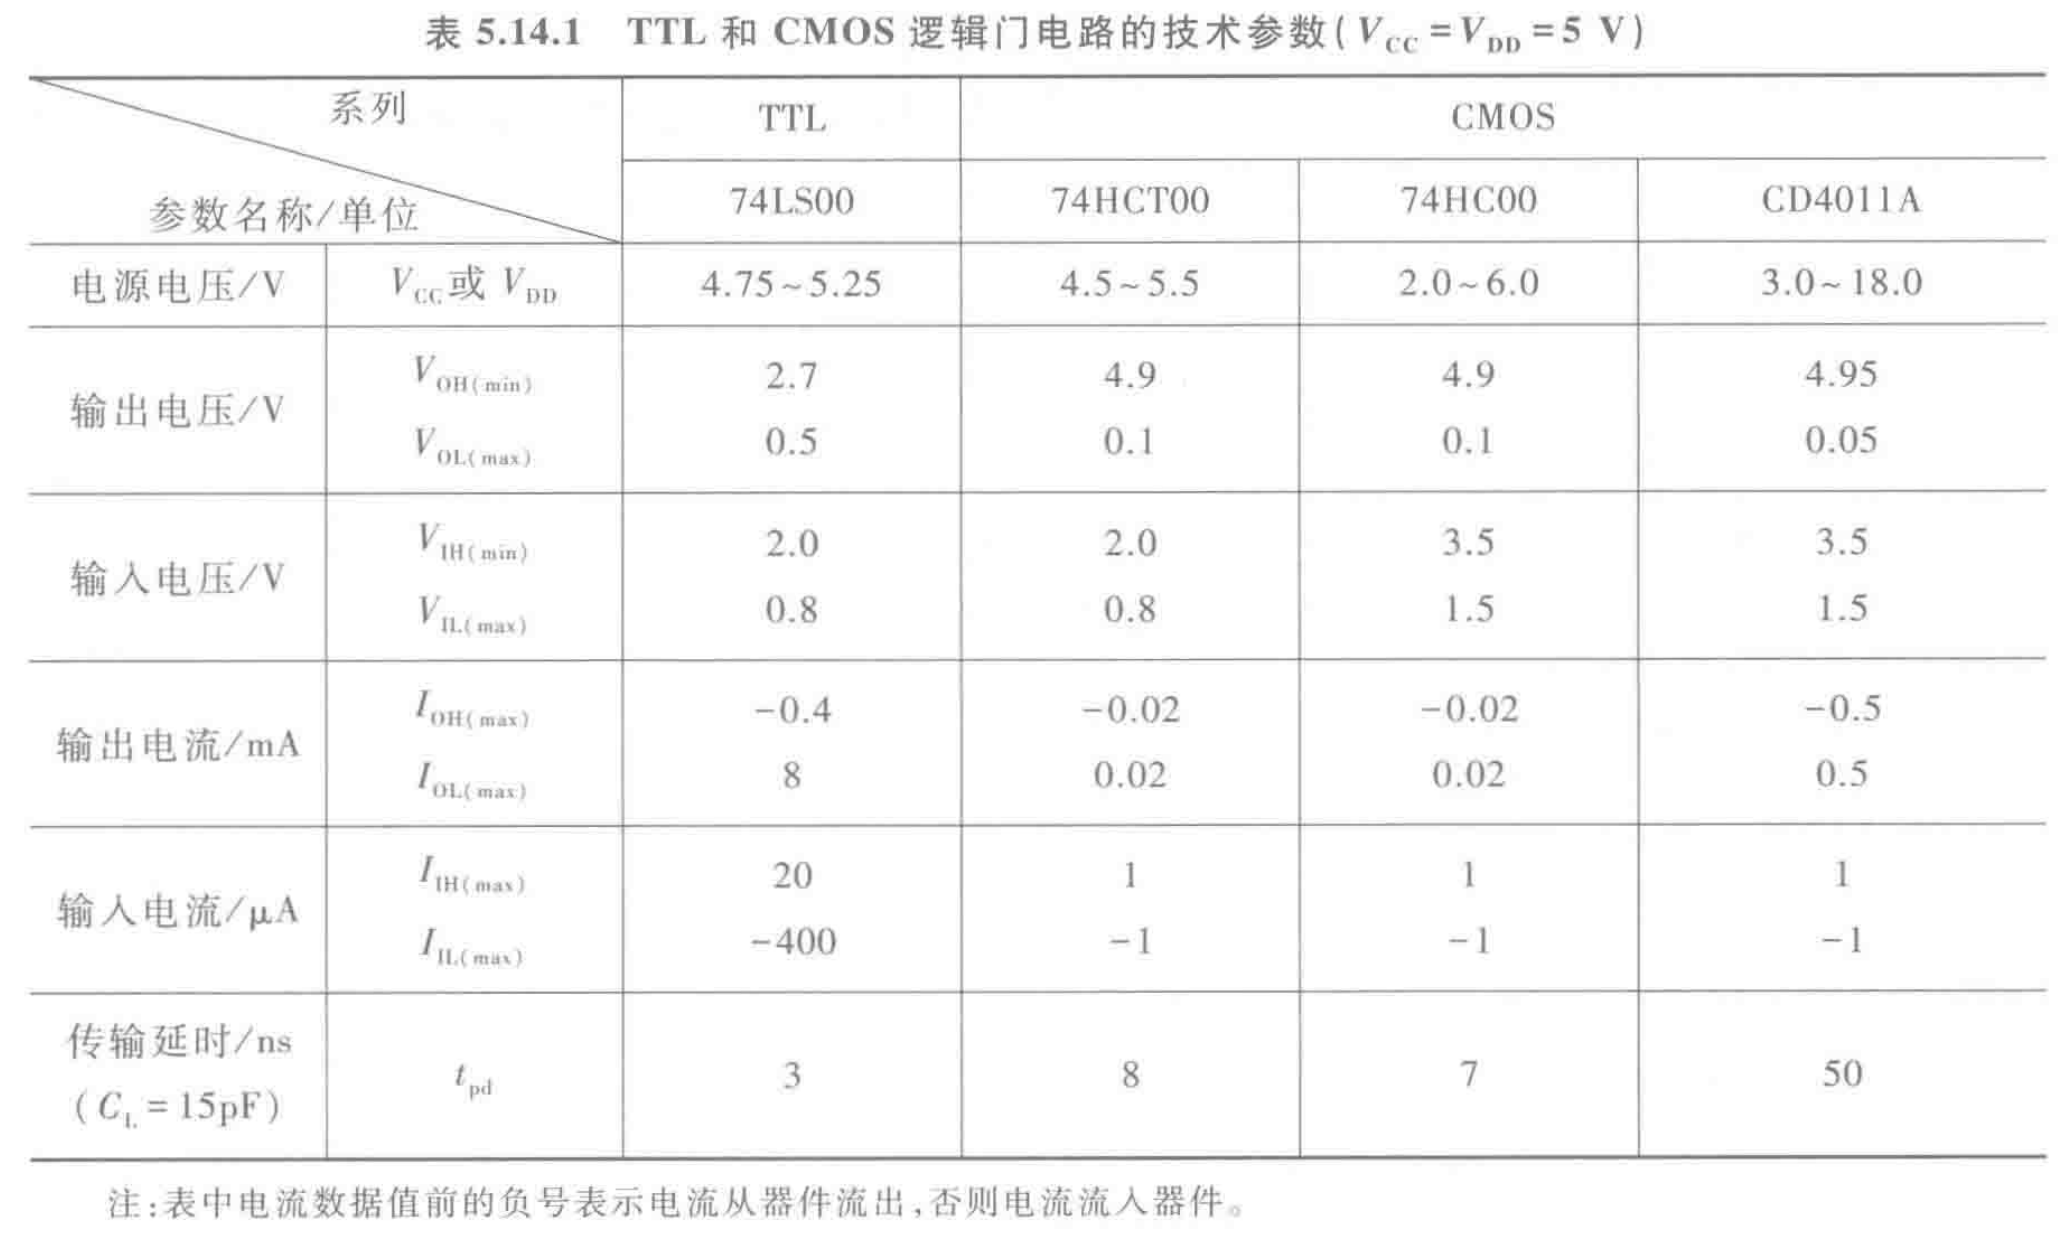
\includegraphics[width=0.82\textwidth]{e6docx_media/media_new/image1.png}
    \caption{逻辑门主要参数参考图}
\end{figure}

\subsection{组合逻辑设计 }
组合逻辑电路设计流程为：逻辑抽象、列真值表、逻辑化简、器件映射和电路实现。逻辑化简的目标是在功能不变前提下减少门数、缩短信号路径并提升可靠性。

TTL/CMOS 门电路使用中需注意：电源稳定、输入端不得悬空、输出端不能违规并联，布线应尽量短以降低干扰。

本实验使用两片 74HC00 设计一位二进制数比较电路，输出三种状态：$L_1(A>B)$、$L_2(A<B)$、$L_3(A=B)$。

\begin{figure}[H]
    \centering
    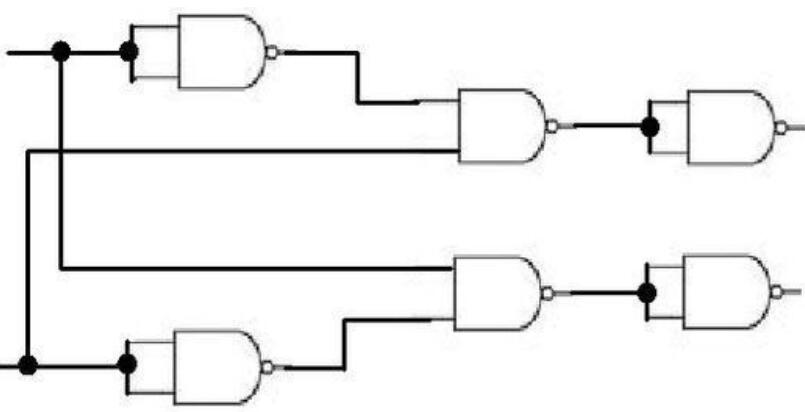
\includegraphics[width=0.75\textwidth]{e6docx_media/media/image13.jpeg}
    \caption{比大小组合逻辑参考电路}
\end{figure}

\section{硬件实验内容}
\subsection{集成逻辑门电路参数测试}
\subsubsection{测 $V_{OH}$}
按下拉电阻法连接测试电路，改变负载条件（空载、510$\Omega$、5.1k$\Omega$），分别测输出高电平。

\begin{figure}[H]
    \centering
    
\includegraphics[width=0.45\textwidth]{e6docx_media/media_new/image2.png}
    \caption{下拉电阻测 $V_{OH}$}
\end{figure}

\subsubsection{测 $V_{OL}$}
按上拉电阻法连接测试电路，改变负载条件（空载、510$\Omega$、5.1k$\Omega$），分别测输出低电平。

\begin{figure}[H]
    \centering
    
\includegraphics[width=0.45\textwidth]{e6docx_media/media_new/image3.png}
    \caption{上拉电阻测 $V_{OL}$}
\end{figure}

\subsubsection{测传输延迟时间 $t_{pd}$}
将多个门串联测总延时，记录上升沿延迟 $t_{pLH}$ 与下降沿延迟 $t_{pHL}$，再计算单个门的平均延迟。

\begin{figure}[H]
    \centering
    
\includegraphics[width=0.75\textwidth]{e6docx_media/media_new/image4.png}
    \caption{传输延迟测试电路}
\end{figure}

\subsection{组合逻辑设计 }
仅使用两片 74HC00，搭建一位二进制比较器。输入端 A、B 分别接高低电平，观察三路 LED 输出：
\begin{itemize}
    \item $L_1$ 亮表示 $A>B$。
    \item $L_2$ 亮表示 $A<B$。
    \item $L_3$ 亮表示 $A=B$。
\end{itemize}

\begin{figure}[H]
    \centering
    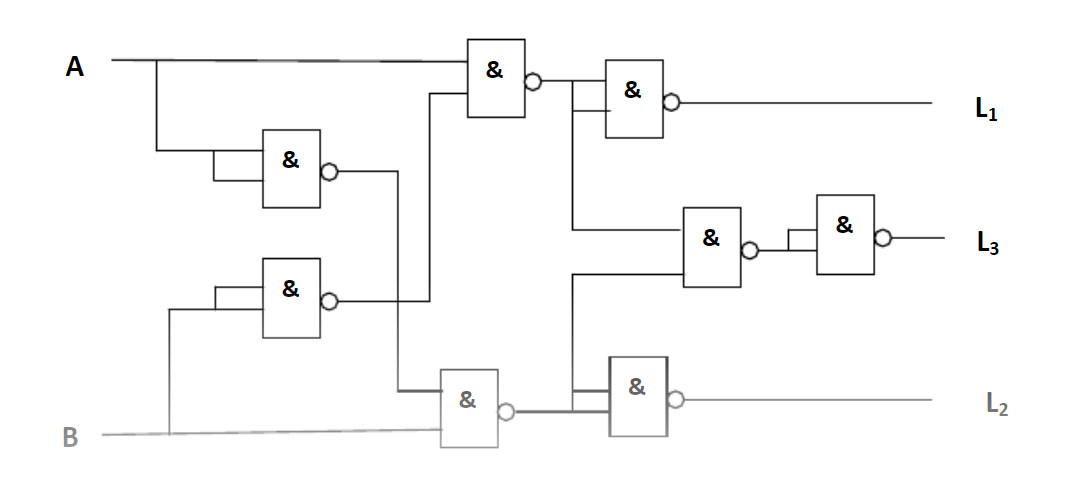
\includegraphics[width=0.78\textwidth]{e6docx_media/media/image14.png}
    \caption{组合逻辑设计 逻辑功能与连线说明}
\end{figure}

\section{硬件实验结果分析}
\subsection{集成逻辑门电路参数测试}
\subsubsection{测量输出高电平 、低电平}

\begin{table}[H]
\centering
\caption{$V_{OH}$、$V_{OL}$ 测试数据}
\renewcommand{\arraystretch}{2.2}
\begin{tabularx}{\textwidth}{|>{\centering\arraybackslash}p{3.6cm}|Y|Y|Y|}
\hline
 & \shortstack{空载} & \shortstack{带载（$5.1k\Omega$）} & \shortstack{带载（$510\Omega$）} \\
\hline
$\displaystyle V_{OH}$ & 20.0mV & 5.06V & \diagbox{}{} \\
\hline
$\displaystyle V_{OL}$ & 5.07V & \diagbox{}{} & 0.321V \\
\hline
\end{tabularx}
\end{table}

\subsubsection{实验数据}

传输延迟测量：$t_{pLH}=116.4\,\text{ns}$，$t_{pHL}=0.13\,\mu\text{s}$。

总延时取平均值约为
\[
 t_{pd(\text{total})}=\frac{t_{pLH}+t_{pHL}}{2}=123.2\,\text{ns}
\]

单个与非门延迟约为
\[
 t_{pd}=\frac{123.2\,\text{ns}}{4}=30.8\,\text{ns}
\]

\subsubsection{结果分析}
空载时测得输出电平受测试方式影响较明显，接入合适负载后输出高、低电平更接近器件实际工作状态。实验中测得 $t_{pd}$ 与手册参数存在偏差，可能由手动游标读数误差引起。

\subsection{组合逻辑设计 }
\subsubsection{实验插板图}
\begin{figure}[H]
    \centering
    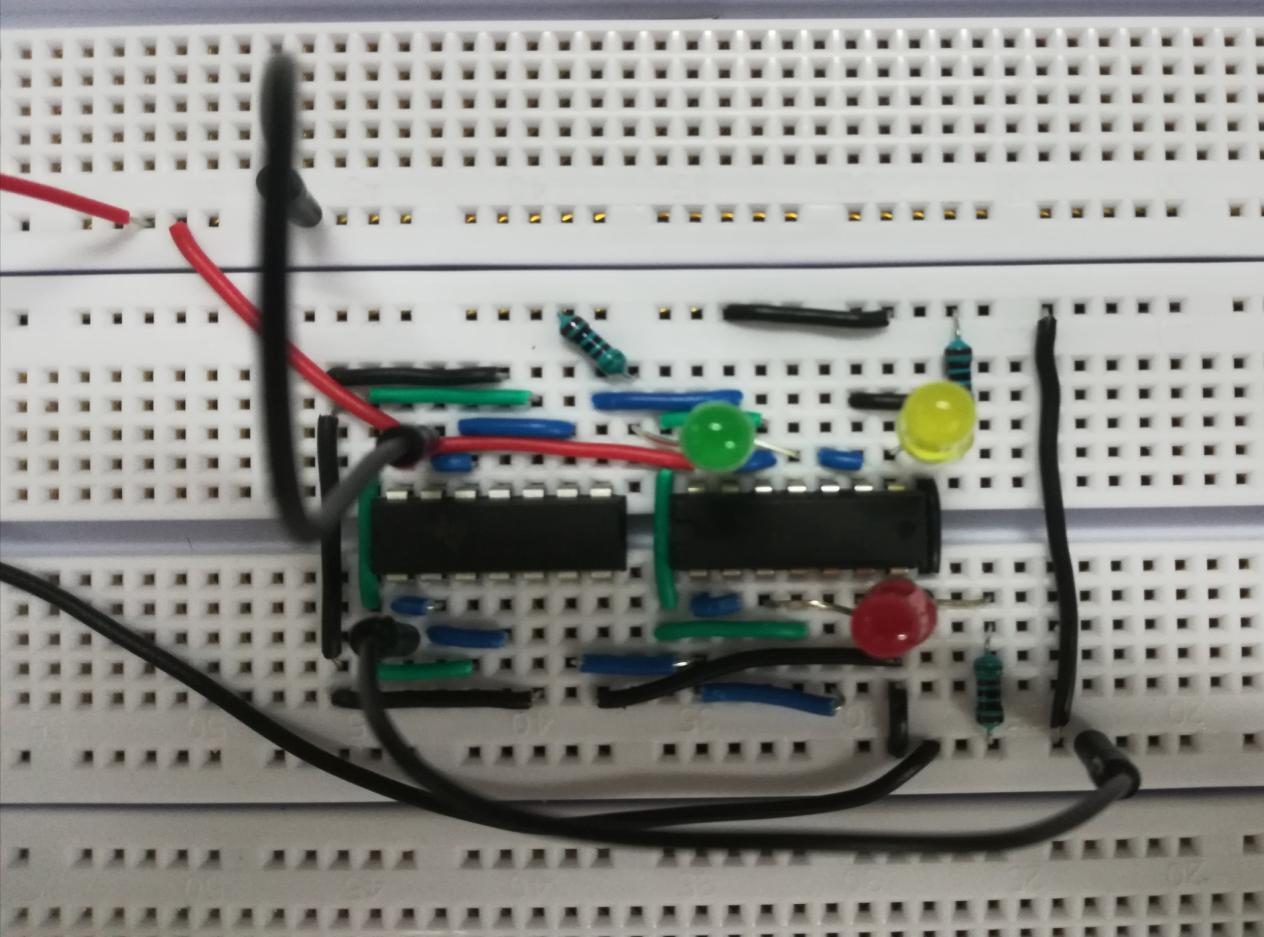
\includegraphics[width=0.75\textwidth]{e6docx_media/media/image15.jpeg}
    \caption{组合逻辑设计 插板图（一）}
\end{figure}

\begin{figure}[H]
    \centering
    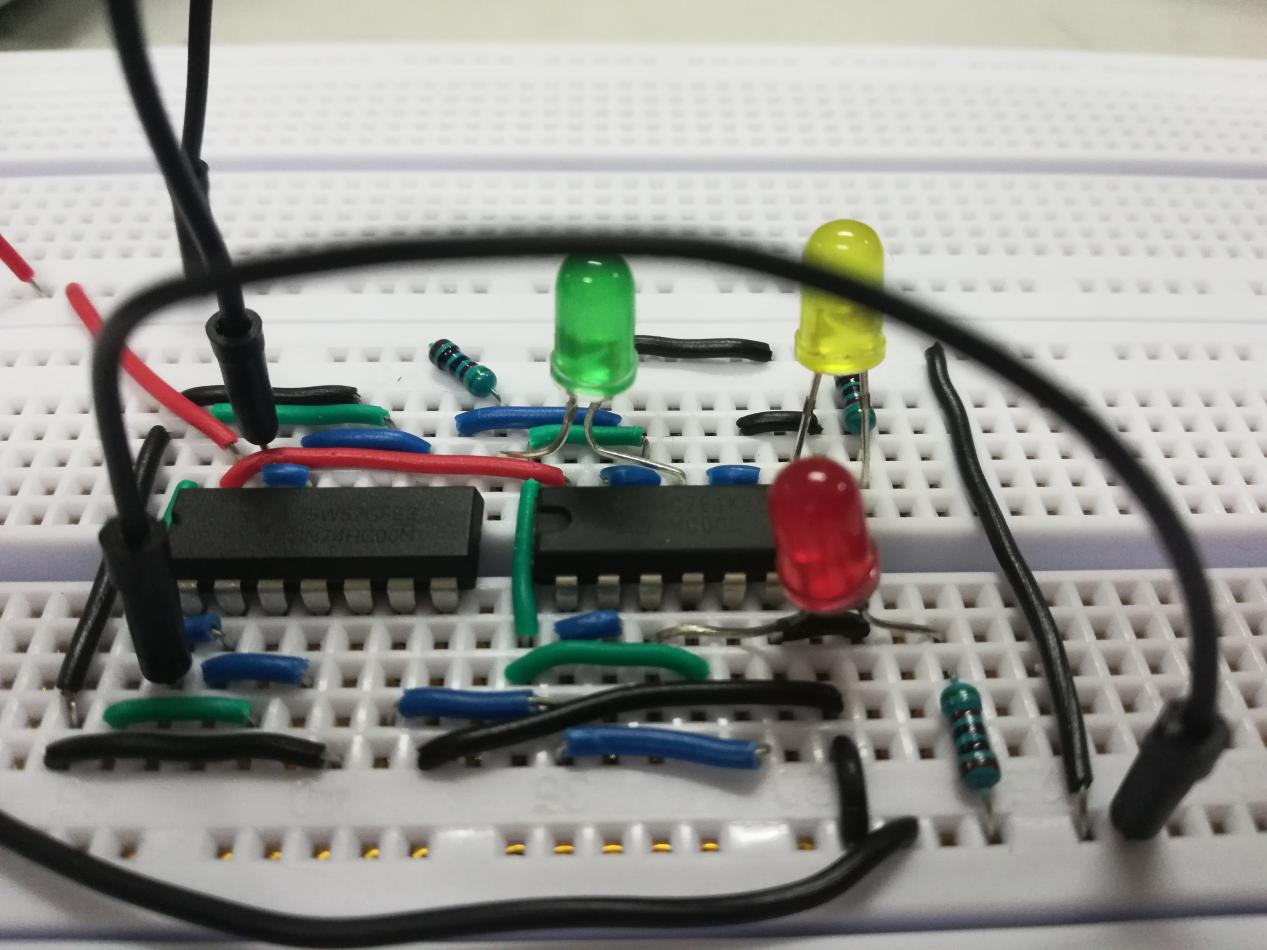
\includegraphics[width=0.75\textwidth]{e6docx_media/media/image16.jpeg}
    \caption{组合逻辑设计 插板图（二）}
\end{figure}

\subsubsection{实验效果图与分析}
\begin{figure}[H]
    \centering
    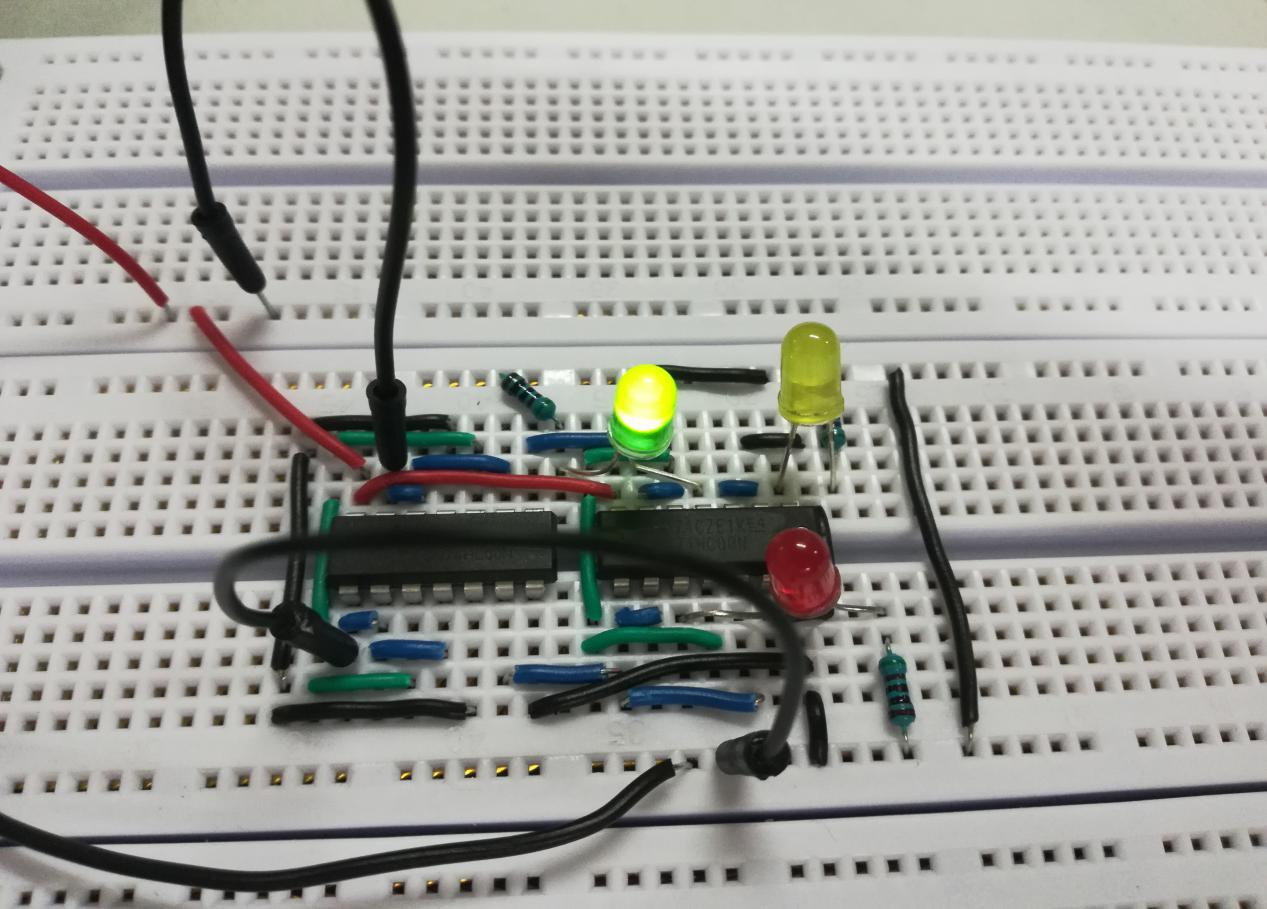
\includegraphics[width=0.75\textwidth]{e6docx_media/media/image17.jpeg}
    \caption{$A>B$ 时（绿灯亮）}
\end{figure}

\begin{figure}[H]
    \centering
    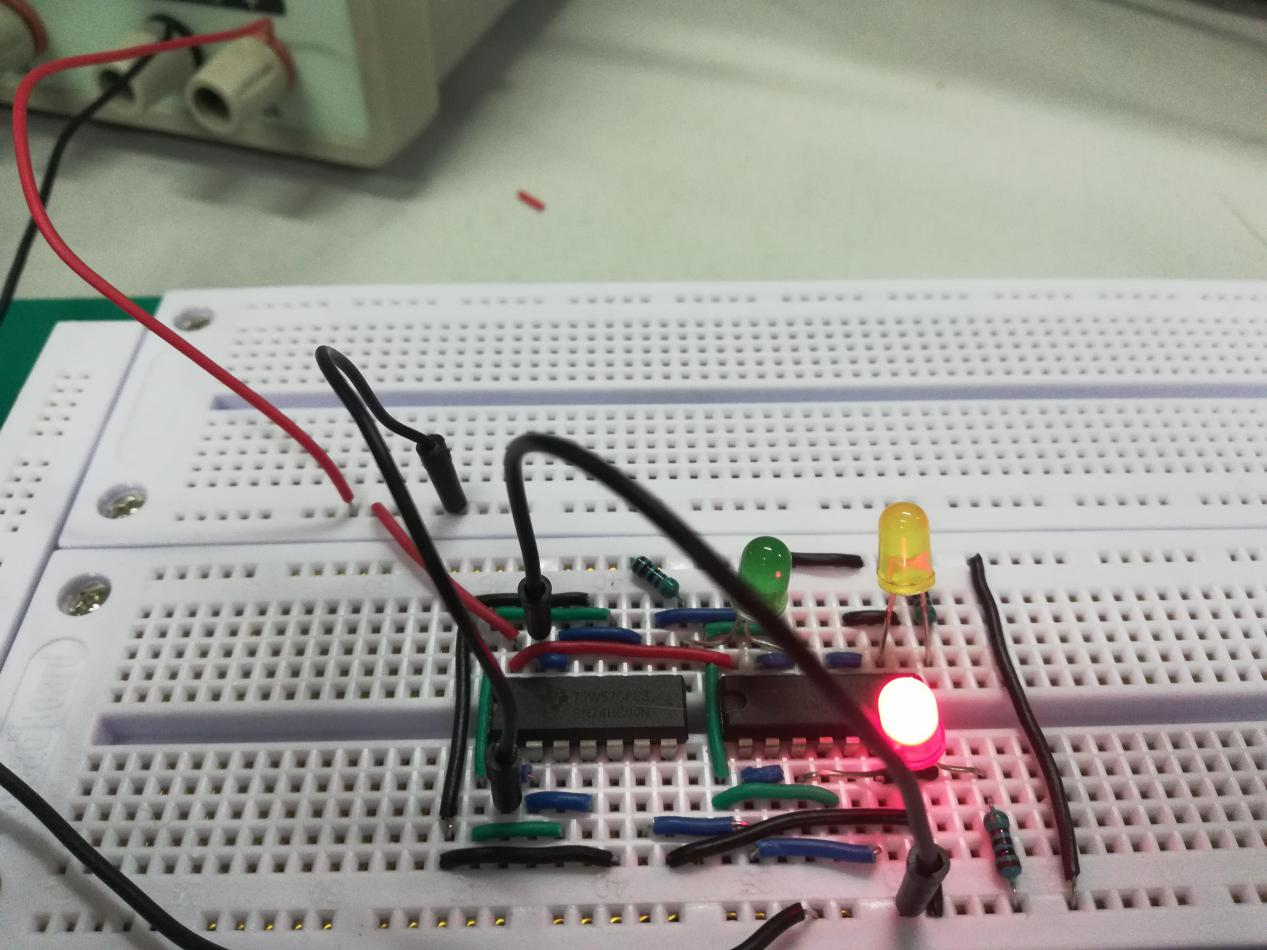
\includegraphics[width=0.75\textwidth]{e6docx_media/media/image18.jpeg}
    \caption{$A<B$ 时（红灯亮）}
\end{figure}

\begin{figure}[H]
    \centering
    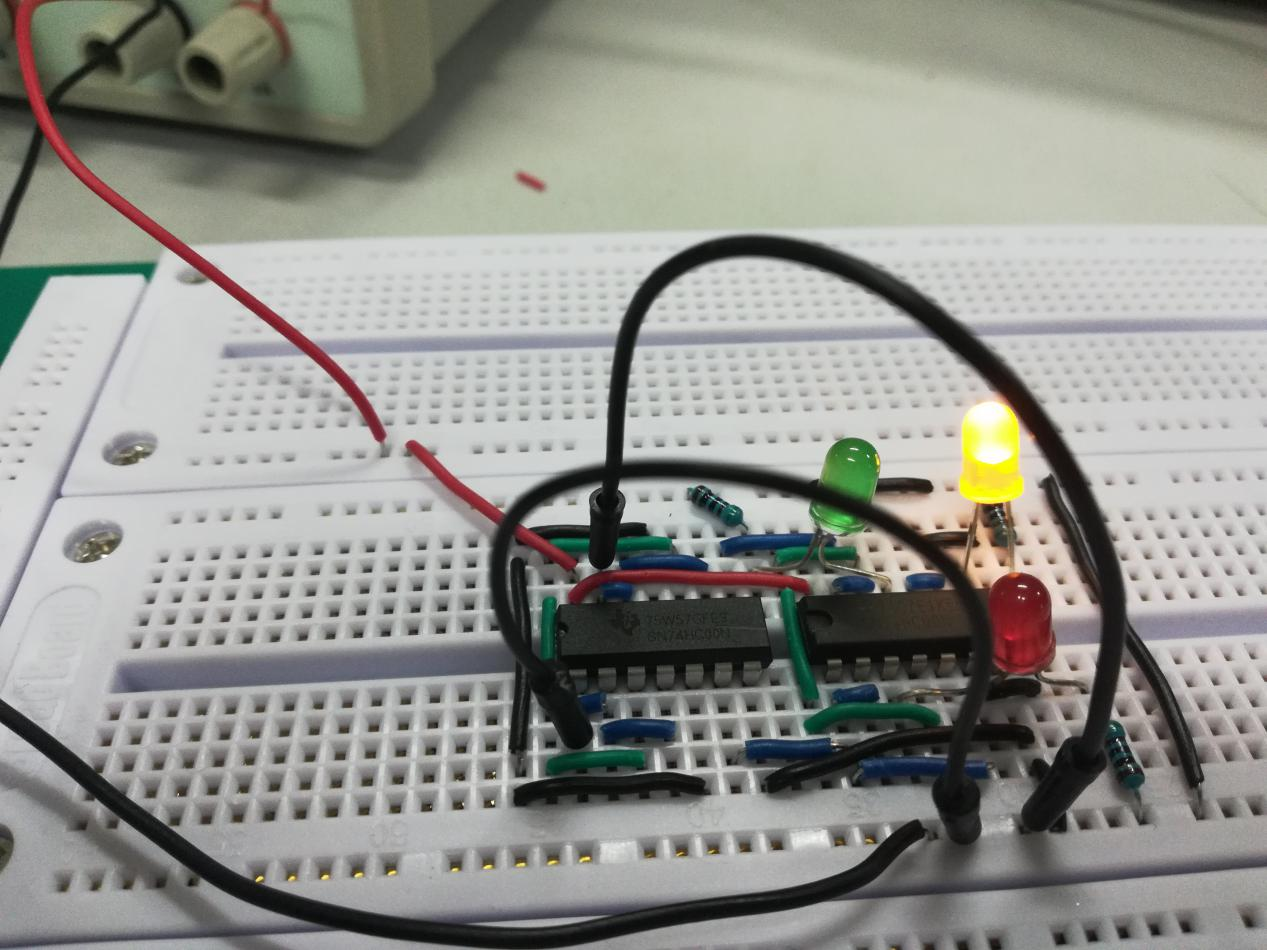
\includegraphics[width=0.75\textwidth]{e6docx_media/media/image19.jpeg}
    \caption{$A=B$ 时（同为低电平，黄灯亮）}
\end{figure}

\begin{figure}[H]
    \centering
    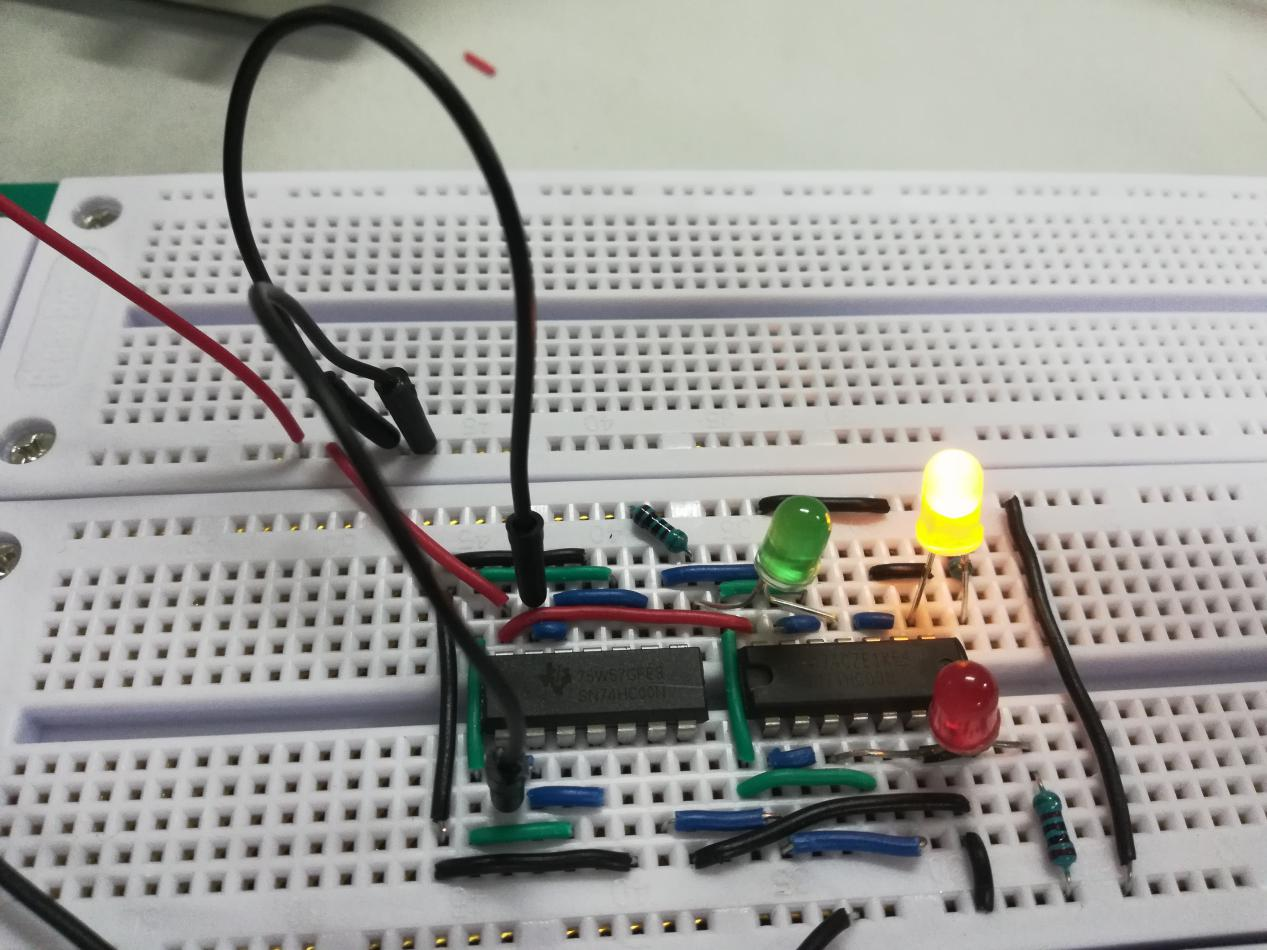
\includegraphics[width=0.75\textwidth]{e6docx_media/media/image20.jpeg}
    \caption{$A=B$ 时（同为高电平，黄灯亮）}
\end{figure}

实验现象与理论一致，电路实现了比较功能。

\section{实验总结}
\subsection{集成逻辑门电路参数测试}
实验过程较顺利，主要完成了逻辑电平与延迟参数的测量。操作中体会到自动测量功能在延迟读数时更稳定、精度更高，可减少人工游标误差。

\subsection{组合逻辑设计 }
实验初期出现 LED 闪烁和状态不稳定，分析为电源引线过长导致干扰较大。将 5V 电源引线缩短后，电路稳定工作，三种比较状态均可正确显示。

\section{思考题}
\subsection{集成逻辑门电路参数测试}
\begin{enumerate}
    \item 当异或门的一个输入端接高电平时，它相当于什么门？

    答：相当于非门。

    \item 用一片 CD4011 可以构成几个非门？几个二输入与门？

    答：可构成四个非门，也可构成两个二输入与门。

    \item 两个普通与非门的输出端并联会产生什么后果？

    答：会形成大电流冲突，可能导致器件损坏。
\end{enumerate}

\subsection{组合逻辑设计 }
\begin{enumerate}
    \item 在设计组合逻辑电路时，为什么要进行逻辑化简？化简依据是什么？

    答：化简是在功能不变前提下进行优化，可减少器件数量、缩短路径并降低成本。化简依据是布尔代数与卡诺图方法。
\end{enumerate}

\end{document}
